% !TEX root = ./Basilisk-Integrators20170724.tex

\section{Test Description and Success Criteria}

As the integrator functionality is not a regular BSK module with specified input/output behavior, the integration can only be tested in an integrated test.
The integrated test employed is located in:\\

{\tt src/tests/scenarios/test\_scenarioIntegrators.py}
\\

\subsection{Test inputs}
Each simulation uses the point-mass spacecraft equations of motion
\begin{equation}
	\ddot{\bm r} = - \frac{\mu}{r^{3}}{\bm r}
\end{equation}
with the initial orbit elements shown in Table~\ref{tbl:oeInitial}.  The only gravitational body considered is Earth.  The simulation time for each case is 3/4 of an orbit period.  Each implemented Integrator method is tested using the above initial conditions and a large time step of 120 seconds.  This large time step makes the integrator errors more easily visible between the integration methods.


\begin{table}[htbp]
	\caption{Initial Spacecraft Ephemeris}
	\label{tbl:oeInitial}
	\centering \fontsize{10}{10}\selectfont
	\begin{tabular}{c | r | r } % Column formatting,
		\hline
		\hline
		Element    & Description & Value \\
		\hline
		$a$      & Semi-Major Axis & 7000km \\
		$e$ & Eccentricity     &  0.0001 \\
		$i$       & Inclination Angle  & 33.3\dg \\
		$\Omega$       & Ascending Node   & 33.3\dg \\
		$\omega$       & Argument of Periapses  & 48.2\dg \\
		$f$       & True Anomaly   & 347.8\dg \\
		\hline
		\hline
	\end{tabular}
\end{table}



\subsection{Test sections}
The same simulation setup is run for each of the integration methods:
\begin{enumerate}
\item The first test uses the default RK4 integration method.  Here the simulation script does not specify the integration method, testing both that the RK4 integrator is the default integration method, and that that the integrator is implemented correctly.

\item The 2nd test uses the RKF45 integration method.

\item The 3rd test used the RK78 integration method.

\item The 4th test uses the Euler's integration method.

\item the 5th test uses Heun's integration method.

\item the 6th test uses the RK3 integration method, whose coefficients are specified through Python.

\item the 7th test uses the (adaptive) Bogacki-Shampine integration method, whose coefficients are specified through Python.

\end{enumerate}

\begin{figure}[t]
	\centerline{
	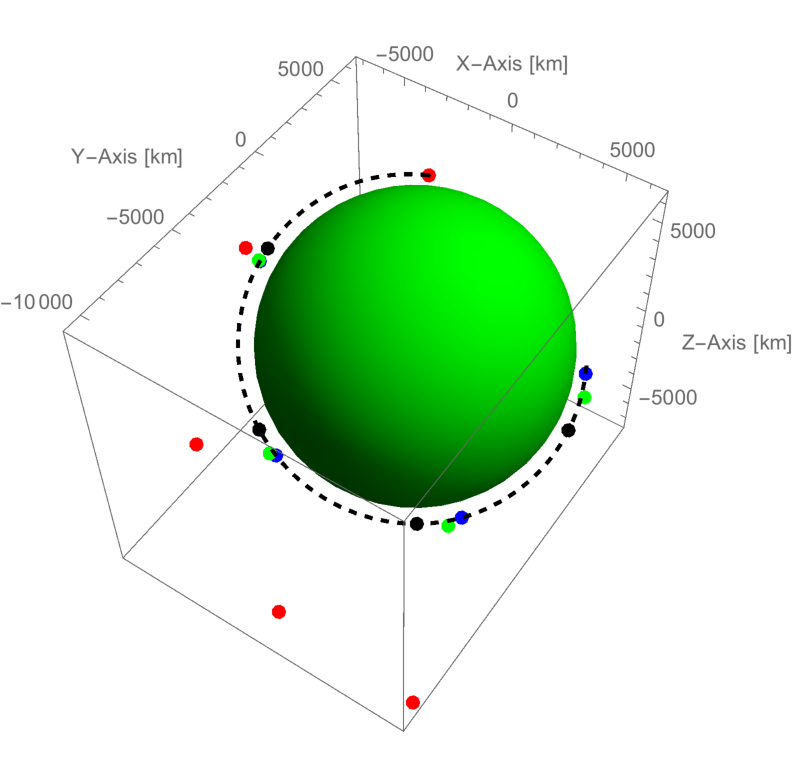
\includegraphics[]{Figures/intResults}
	}
	\caption{Illustration of the true orbit position samples (Black) versus the RK4 (Blue), RK2 (Green) and RK1 (Red) integration results.}
	\label{fig:intResults}
\end{figure}
The resulting data points are illustrated in Figure~\ref{fig:intResults}.  The large 120 second time step causes all the integration methods to significantly deviate from the truth locations (shown in black).  The integrated validation test ensures that the BSK integrations yield the same integration corruptions to validate the mathematical implementation.

\subsection{Test success criteria}
For the fixed-step integrators, the integrated position states are checked at 5 even data points along the simulation time againt pre-computed truth answers.  These truth answers were generated in Mathematica implementing the same initial conditions, and replicating the integration math.    The accuracy threshold is set to 1 meter, a small value compared to the 7,000,000 meter near-circular orbit radius.

For the variable-step (adaptive) integrators, only the final position is checked. This position is compared to the analytical 2-body solution, and the error is constrained to be lower than one meter. This guarantees that the adaptive integrators can achieve very high accuracy irrespective of the user-provided step size.

\section{Test Parameters}
Three tests are run controlled through a single test parameter called {\tt integratorCase}.  The possible values are shown in Table~\ref{tbl:intCases}.

\begin{table}[htbp]
	\caption{Error tolerance for each test.}
	\label{tbl:intCases}
	\centering \fontsize{10}{10}\selectfont
	\begin{tabular}{ c | c } % Column formatting,
		\hline\hline
		\textbf{Test}   	      	               & \textbf{Tolerated Error} 						           \\ \hline
		``rk4"                           & 1 meter	  \\
		``rkf45"                           & 1 meter	  \\
		``rkf78"                           & 1 meter	  \\
		``euler"                           & 1 meter	  \\
		``rk2"                           & 1 meter	  \\
		``rk3"                           & 1 meter	  \\
		``bogackiShampine"                           & 1 meter	  \\
		\hline\hline
	\end{tabular}
\end{table}

\section{Test Results}
All integration checks within the integrated test {\tt scenarios/test\_scenarioIntegrators.py} passed.  Table~\ref{tbl:intResults} shows the test results, while Figure~\ref{fig:intResults} shows the resulting trajectories for each integration test.

\input{AutoTeX/scenarioIntegrators.tex}

\begin{table}[h]
	\caption{Integration test results.}
	\label{tbl:intResults}
	\centering \fontsize{10}{10}\selectfont
	\begin{tabular}{c | c | p{4in} } % Column formatting,
		\hline\hline
		\textbf{Test} 			& \textbf{Pass/Fail} 	 & \textbf{BSK Error Notes}
		\\ \hline
		``rk4"		  	&
		\input{AutoTex/IntegratorsTestMsg-rk4}      	  &
		\input{AutoTex/IntegratorsMsg-rk4}
		\\ \hline
		``rkf45"		  	&
		\input{AutoTex/IntegratorsTestMsg-rkf45}      	  &
		\input{AutoTex/IntegratorsMsg-rkf45}
		\\ \hline
		``rkf78"		  	&
		\input{AutoTex/IntegratorsTestMsg-rkf78}      	  &
		\input{AutoTex/IntegratorsMsg-rkf78}
		\\ \hline
		``euler''	   	           	&
		\input{AutoTex/IntegratorsTestMsg-euler}           		&      
		\input{AutoTex/IntegratorsMsg-euler}  
		\\ \hline
		``rk2''      	&
		\input{AutoTex/IntegratorsTestMsg-rk2}
		&
		\input{AutoTex/IntegratorsMsg-rk2}
		\\ \hline
		``rk3''      	&
		\input{AutoTex/IntegratorsTestMsg-rk3}
		&
		\input{AutoTex/IntegratorsMsg-rk3}
		\\ \hline
		``bogackiShampine''      	&
		\input{AutoTex/IntegratorsTestMsg-bogackiShampine}
		&
		\input{AutoTex/IntegratorsMsg-bogackiShampine}
		\\
		\hline\hline
	\end{tabular}
\end{table}
